\section{Практическая часть.}

2.2 Написать функцию, вычисляющую гипотенузу прямоугольного треугольника по заданным катетам и составить диаграмму ее вычисления.

\begin{lstlisting}
(DEFUN C (A B) (SQRT (+ (* A A) (* B B))))
\end{lstlisting}

\begin{figure}[ht!]
 	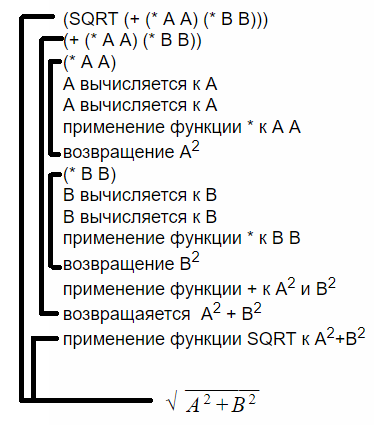
\includegraphics[width=1.1\textwidth]{1.PNG}
 	\caption{Диаграмма функции 2.2.}
 \end{figure}

3.1 - Написать функцию, которая принимает целое число и возвращает первое четное число, не меньшее аргумента.
 \begin{lstlisting}
 (DEFUN F(X) (IF (ODD X) (+ X) (+ X 2)))
\end{lstlisting}
3.2 - Написать функцию, которая принимает число и возвращает число, того же знака, но с модулем на 1 больше аргумента.
 \begin{lstlisting}
 (DEFUN F(X) (IF (> X 0) (+ X 1) (- X 1)))
\end{lstlisting}
3.3 - Написать функцию, которая принимает два числа и возвращает список из этих чисел, расположенный по возрастанию.
 \begin{lstlisting}
 (DEFUN F(X Y) (IF (< X Y) (LIST X Y) (LIST Y X)))
\end{lstlisting}
3.4 - Написать функцию, которая принимает три числа и возвращает Т только тогда, когда первое число расположено между первым и вторым.
 \begin{lstlisting}
 (DEFUN F(X Y Z) (OR (AND (> X Y) (< X Z) (AND (> X Z) (< X Y)))))
\end{lstlisting}
2.7 - Написать функцию, которая переводит температуру в системе Фаренгейта в температуру по Цельсию. Как бы назывался роман Р. Брэдбери "+451 по Фаренгейту" в системе по Цельсию? 
 \begin{lstlisting}
 (DEFUN F_TO_C (TEMP) (* (/ 5 9) (- TEMP 320)))

 (F_TO_C 451) => 72.77778
\end{lstlisting}
2.8 - Что получится при вычислении выражений?
 \begin{lstlisting}
 (LIST 'CONS T NIL) => (CONS T NIL)
 (EVAL (EVAL (LIST 'CONS T NIL))) => UNDERFINED FUNCTION T
 (APPLY #'CONS '(T NIL)) => (T)
 (LIST 'EVAL NIL) => (EVAL NIL)
 (EVAL (LIST 'CONS T NIL)) => (T)
 (EVAL NIL) => NIL
 (EVAL (LIST 'EVAL NIL)) => NIL
\end{lstlisting}
  